\subsection{Генератор синтаксических анализаторов Yacc} \label{sub117}

\textit{Yacc}~--- компьютерная программа, служащая стандартным генератором синтаксических анализаторов в~Unix-системах. Название является акронимом \textit{<<Yet Another Compiler Compiler>>} (<<ещё один компилятор компиляторов>>)~\cite{Johnson1975}. Yacc генерирует синтаксический анализатор на~основе аналитической грамматики, описанной в~нотации Бэкуса-Наура или контекстно-свободной грамматики. На выходе Yacc выдаётся код на~языке программирования~С.

Поскольку синтаксический анализатор, генерируемый с~помощью Yacc, требует использования лексического анализатора, то~часто он используется совместно с~генератором лексических анализаторов, в~большинстве случаев это Lex либо Flex. 

Создание транслятора с~использованием Yacc схематично показано на~рис.~\ref{img:yacc}. Вначале создаётся файл, например, \texttt{translate.y}, содержащий Yacc-спецификацию разрабатываемого транслятора. Затем этот файл преобразуется в~программу \texttt{t.tab.c} на~языке C, которая является синтаксическим анализатором, который реализует восходящий тип разбора. На~вход скомпилированной программе \texttt{a.out} поступает поток токенов, а~результатом работы становится синтаксическое дерево разбора \cite{Aho2003}.

\begin{figure}[ht]
	\centering
	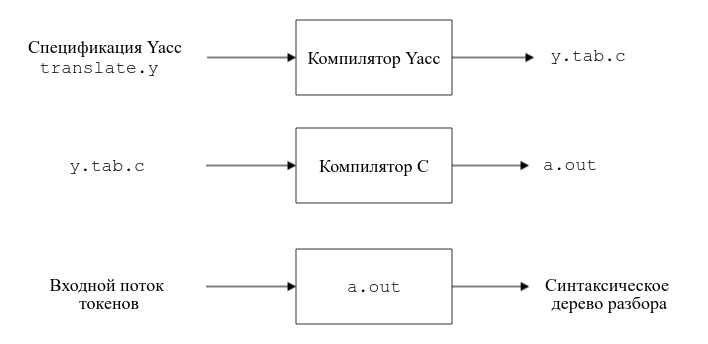
\includegraphics [scale=0.65] {yacc}
	\caption{Создание транслятора с помощью Yacc}
	\label{img:yacc}
\end{figure}

\textit{GNU(<<GNU~is~Not~Unix>>)}-альтернативой Yacc служит \textit{Bison}, он~практически полностью совместим с~Yacc, за~исключением небольших синтаксических дополнений и~флагов запуска программы~\cite{Levine1992}. 
